\section{The first selection and path--level intersections}
\label{sec:selection}

This section has two outputs.  First, we select a countable compatible
list of real barriers and a countable set of ends $S$.  In every later
compatible finite-transfer limit, each component indexed by $B\setminus S$
will be a point.  The selection rests on a planar crossing argument:
uncountably many endpoints without small barriers would give laws whose forced
intersections contradict their occupation and hit bounds.  Second, we
prove that a path law has finite expected intersection count with a
generic prior level union and avoids its entire free dust subset.  This
will supply the intersection estimates for the period coordinates.

We retain $g_\mu$ for a law's mean domain arclength density, $n_\mu$
for its expected visit counts including the final time, and $m_\mu$ for
its hit probabilities.  Thus $m_\mu\le n_\mu$.
Theorem~\ref{thm:positive-law} bounds $m_\mu$ on all of $B$ and
$n_\mu$ on the prescribed countable set $D_*$; the distinction will
matter in the intersection estimates.

\subsection{Point avoidance and intersections of two laws}

We begin by ruling out atoms at physical domain points.  The corresponding
statement for dust points requires the residual incidence constraints and
the absolutely continuous tag distributions.

\begin{lemma}[Avoidance of domain points]
\label{lem:point-avoidance}
Let $\mu$ be a law of paths ending in $B$, with expected domain arclength
occupation $g_\mu\,\dd a$ and $g_\mu\in L^2(G)$.  Every fixed point of $G$ is
visited with probability zero.  In particular, if all paths start outside
the closure of a dust disk $U$ and end in $U\cap B$, their last-hit
locations on $\partial U$ have an atomless distribution.
\end{lemma}

\begin{proof}
Fix $x\in G$.  In a physical coordinate disk about $x$, with coordinate
$z(x)=0$, choose $r_0>0$ so that its closed $r_0$-disk lies in $G$.
Consider the nonnegative density, defined to be zero at $x$ and outside
the indicated punctured disk,
\[
 \rho(z)=\frac{\ind_{\{0<|z|<r_0/e\}}}
 {|z|\log(r_0/|z|)}.
\]
The smooth spherical length factor is bounded above and below on this
disk, and
\[
 \int_0^{r_0/e}\frac{\dd r}{r\log^2(r_0/r)}<\infty,
 \qquad
 \int_0^{r_0/e}\frac{\dd r}{r\log(r_0/r)}=\infty.
\]
Consequently $\rho\in L^2(G,\dd a)$, while every path that visits $x$ and
subsequently leaves this coordinate disk has infinite $\rho$-length on
its domain times.  To see the latter assertion without any regularity at
the hitting time, stop between the circles of radii $a$ and $r_0/e$ and
apply ordinary variation to the radial coordinate, then let $a\downarrow0$.
Every path under consideration ends in $B$ and therefore must leave this
disk after a visit to $x$.  On the other hand,
\[
 \E_\mu\int_{\gamma^{-1}(G)}\rho(\gamma)\,\dd s
 =\int_G\rho g_\mu\,\dd a
 \le \|\rho\|_2\|g_\mu\|_2<\infty.
\]
This proves point avoidance.

For a path from outside $\overline U$ to $U\cap B$, the set of hitting
times of $\partial U$ is a nonempty compact set whose maximum is less
than $1$.  The path lies strictly inside $U$ after that maximum.  An atom
at a given last-hit location would give positive probability of visiting
that fixed point of $\partial U\subset G$, which has just been excluded.
\end{proof}

\begin{lemma}[Removal of diffuse dust intersections]
\label{lem:diffuse-intersections}
Fix a countable prior coordinate list satisfying \textup{(P)}, with flag
set $\Sigma$.  Let $\xi$ and $\mu$ be laws on allowed tagged paths for
this list, and put $A_\xi=\{s\in B:m_\xi(s)>0\}$.  Assume that
\[
 m_\xi,m_\mu\in\ell^2(B),\qquad
 n_\xi|_\Sigma\in\ell^2(\Sigma),\qquad
 n_\mu|_{A_\xi}\in\ell^2(A_\xi).
\]
Assume also that, for each law and every slot and tag type, the corresponding
tuple subprobability is absolutely continuous with respect to Haar measure
on its tuple torus.  Finally, assume that $\xi$ is imposed as an earlier
law in the path system for $\mu$.
For independent samples from $\xi$ and $\mu$, almost surely,
\[
 \gamma_\xi([0,1])\cap\gamma_\mu([0,1])\cap B
 \subset
 \Sigma\cup\{m_\xi>0\}\cup\{m_\mu>0\}.
\]
In particular all common dust visits are confined, up to a null event,
to a countable set.
\end{lemma}

These hypotheses hold for the laws used below.  Indeed,
Theorem~\ref{thm:positive-law} supplies the hit and tuple bounds;
the prescribed countable set for $\xi$ contains $\Sigma$, and that
for $\mu$ contains the hit support of each imposed earlier law.

\begin{proof}
There are three cases to control: a residual contact of the later path,
a residual contact of the earlier path with a later tag, and a contact
between two tags.

\smallskip\noindent\emph{Residual contacts of the later path.}
Let $P_N$ be the finite deletions exhausting $A_\xi$ in the residual
intersection constraint.  With
$Z_\gamma$ denoting the residual dust times of a tagged path, that
constraint, independence, and Tonelli's theorem give
\begin{align*}
 &\Prob\bigl(
 \gamma_\xi([0,1])\cap
 (\gamma_\mu(Z_{\gamma_\mu})\setminus P_N)\ne\varnothing
 \bigr)\\
 &\hspace{15mm}\le
 \sum_{s\in A_\xi\setminus P_N}m_\xi(s)n_\mu(s)
 \le
 \|m_\xi\ind_{A_\xi\setminus P_N}\|_{\ell^2}
 \|n_\mu|_{A_\xi}\|_{\ell^2}.
\end{align*}
The last factor is finite by the assumed count bound, and the first
tends to zero.  Thus any meeting at a residual time of the later path
occurs in $A_\xi$, almost surely.

\smallskip\noindent\emph{An earlier residual contact with a later tag.}
Next fix a prior coordinate $i$, and delete finite sets exhausting
$\Sigma$ in its residual level constraint.  Almost surely the weighted
sum of visits of $\gamma_\xi$ against $a_i$ is finite, since its
expectation is at most
\[
 \|a_i\|_{\ell^2}\|n_\xi|_\Sigma\|_{\ell^2}.
\]
The deleted tails of this sum tend to zero.  It follows directly from
the residual level constraint that
\[
 \bigl|\{t\in\T:
 H_i(t)\cap(\gamma_\xi(Z_{\gamma_\xi})\setminus\Sigma)
 \ne\varnothing\}\bigr|=0
 \quad\text{almost surely}.
\]
This assertion holds simultaneously for all prior labels.  Conditional
on an earlier path with this property, a tag of the independent later
path cannot meet its residual image off $\Sigma$: each coordinate
level in the tag has an absolutely continuous marginal distribution.
There are only countably many tag slots and types, so all such meetings
are excluded simultaneously.

\smallskip\noindent\emph{Contacts between two tags.}
It remains to exclude a free common point lying on a tag of each path.
For any fixed pair of slots and types, their two tuples are independent
and absolutely continuous with respect to their level product measures.
We can therefore assume simultaneously that all required instances of
\textup{(P)} hold and that levels belonging to the same label in the two
tuples are distinct.  At a free common point $x$, choose the largest
label $j$ among the levels from either tag that actually contain $x$.
The unique trace at $x$ implies that label $j$ can occur at $x$ in only
one of the two tags.  In the other tag, every level present at $x$ has
label less than $j$.

Here the other tag supplies a nondegenerate continuum through $x$ in
those lower levels.  Indeed its image is connected and nonconstant.
Choose a compact parameter subinterval within the tag whose image
contains both $x$ and another point.  Level sets in its finite union
that miss $x$ miss some neighborhood of $x$, by closedness.  Boundary
bumping in a sufficiently small closed neighborhood now gives a
nondegenerate subcontinuum through $x$ using only the levels present
there.  This contradicts \textup{(P)} for label $j$.

All these assertions hold simultaneously for the countably many pairs
of slots, types, and sublists.  The incidence events are Borel or
analytic by the path coding and compact level graphs; completed product
measures therefore justify the conditioning and Fubini arguments.
\end{proof}

\subsection{The crossing argument}

We now compare two consequences of having many unavailable endpoints.
Four alternating collar starts force an intersection, while localization
of the law bounds makes each possible cross-pair intersection unlikely.

\begin{theorem}[Countably many unavailable endpoints]
\label{thm:countable-exceptions}
Fix any countable coordinate list satisfying \textup{(P)}, and fix
$\beta>0$.  In the ungated endpoint problem with
\[
 E=\{3R\le |z|\le4R\},
 \qquad E_* =\{|z|=7R/2\},
\]
there are at most countably many $b\in B$ for which no compatible real
barrier $u$ is available with
\[
 \|\dd u\|_2+\|a_u\|_{\ell^2(B)}<\beta.
\]
Availability permits a countable enlargement of the flags.  The
prescribed collar sequence may start arbitrarily deep, and the barrier
is required to equal one on some collar of that sequence.
\end{theorem}

\begin{proof}
\emph{A common collar for uncountably many laws.}
Suppose the unavailable endpoints form an uncountable set.  Choose
distinct such endpoints $b_\alpha$, $\alpha<\omega_1$.  Recursively apply
Theorem~\ref{thm:positive-law} to obtain a law $\mu_\alpha$ from $E$ to
$b_\alpha$ at first arrival.  At stage $\alpha$, impose all the earlier
laws in the residual intersection constraint.  This is an admissible
countable collection because $\alpha$ is countable.  The coordinate
list and its flags remain fixed throughout this recursion.

Fix a number $\delta>0$, to be made small below.  For each endpoint
$p=b_\alpha$, shrinking its exhaustion disk gives
\begin{equation}
 \label{eq:small-law-tail}
 \|g_{\mu_p}\|_{2,U\cap G}<\delta,
 \qquad
 \|m_{\mu_p}|_{(U\cap B)\setminus\{p\}}\|_{\ell^2}<\delta
\end{equation}
for some exhaustion disk $U$ containing $p$.  The first assertion is
absolute continuity of the energy integral, since the disks shrink to
a point outside $G$.  The second is the analogous tail property of a
square-summable family after omitting its value at $p$.  There are only
countably many disks in the exhaustion.  Hence one common $U$ satisfies
Equation~\eqref{eq:small-law-tail} for uncountably many of the chosen
endpoints and their laws.

\smallskip\noindent\emph{Alternating connections.}
For each of these laws, take the last-hit location on $\partial U$.
Its distribution is atomless by Lemma~\ref{lem:point-avoidance}.
Consequently there are four pairwise disjoint arcs $I_1,I_2,I_3,I_4$ on
$\partial U$, listed in circular order, each having probability at least $1/10$.
The arcs can be chosen from a fixed countable family: use any fixed
parametrization of the circle and endpoints in a countable dense set,
choosing slightly smaller quantile arcs before this approximation.
After another uncountable restriction the same ordered four arcs work
for every law.  Choose an earlier endpoint $p$ and a later endpoint
$q$ from this subfamily.

Independently sample two paths to $p$ and two paths to $q$.  With
probability at least $10^{-4}$ their last-hit locations fall,
respectively, in $I_1$ and $I_3$ for the $p$-paths and $I_2$ and
$I_4$ for the $q$-paths.  The tails after these hits lie strictly inside
$U$, apart from their initial points.  Concatenating the two tails
through $p$ gives a connection between its two boundary locations, and
likewise for $q$.  Each connection contains a simple arc between its
boundary endpoints.  Jordan separation in the closed disk
$\overline U$ forces the two connections to intersect in $U$; see
Figure~\ref{fig:crossing}.
Thus this event entails an intersection in $U$ of one of the four
independent cross-pairs consisting of a $p$-path and a $q$-path.

\begin{figure}[tb]
\centering
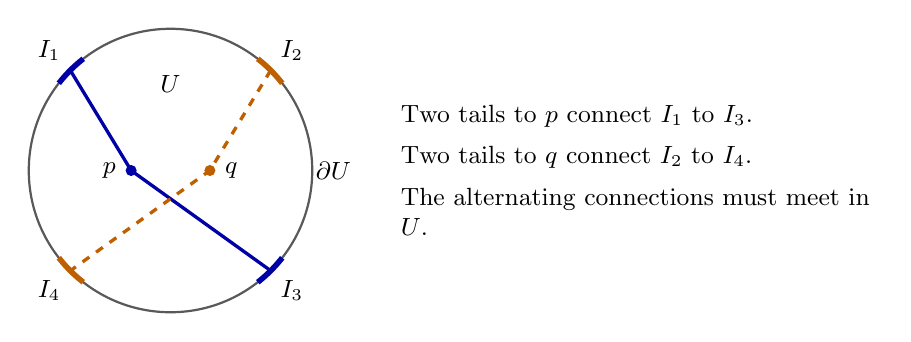
\begin{tikzpicture}[x=1cm,y=1cm,font=\small]
 \draw[black!65,line width=.8pt] (0,0) circle (1.8);
 \draw[blue!65!black,line width=2pt]
 (128:1.8) arc[start angle=128,end angle=142,radius=1.8];
 \draw[orange!75!black,line width=2pt]
 (38:1.8) arc[start angle=38,end angle=52,radius=1.8];
 \draw[blue!65!black,line width=2pt]
 (308:1.8) arc[start angle=308,end angle=322,radius=1.8];
 \draw[orange!75!black,line width=2pt]
 (218:1.8) arc[start angle=218,end angle=232,radius=1.8];
 \node at (2.07,0) {$\partial U$};
 \node at (0,1.1) {$U$};
 \draw[blue!65!black,line width=1.2pt]
 (-1.273,1.273)--(-.5,0)--(1.273,-1.273);
 \draw[orange!75!black,line width=1.2pt,dashed]
 (1.273,1.273)--(.5,0)--(-1.273,-1.273);
 \fill[blue!65!black] (-.5,0) circle (2pt);
 \fill[orange!75!black] (.5,0) circle (2pt);
 \node[left,xshift=-2pt] at (-.5,0) {$p$};
 \node[right,xshift=2pt] at (.5,0) {$q$};
 \node[above left] at (-1.273,1.273) {$I_1$};
 \node[above right] at (1.273,1.273) {$I_2$};
 \node[below right] at (1.273,-1.273) {$I_3$};
 \node[below left] at (-1.273,-1.273) {$I_4$};
 \node[align=left,text width=6cm,anchor=west] at (2.8,0)
 {Two tails to $p$ connect $I_1$ to $I_3$.\\[4pt]
  Two tails to $q$ connect $I_2$ to $I_4$.\\[4pt]
  The alternating connections must meet in $U$.};
\end{tikzpicture}
\caption{The four-path crossing in the quotient disk $U$.
The four boundary arcs occur in cyclic order. After diffuse dust
contacts have been removed, the probability of any required meeting
is bounded by the occupation and hit estimates.}
\label{fig:crossing}
\end{figure}


\smallskip\noindent\emph{Dust intersections.}
We estimate the probability of such a cross-pair intersection.
Lemma~\ref{lem:diffuse-intersections} removes all dust meetings outside
a countable set.  Points in that set with zero hit probability for
either law can also be discarded.  Independence and the union bound
therefore give
\begin{align}
 \label{eq:dust-meeting-bound}
 \Prob(\text{a common visit in }U\cap B)
 &\le \sum_{s\in U\cap B}m_{\mu_p}(s)m_{\mu_q}(s)\notag\\
 &\le m_{\mu_q}(p)+m_{\mu_p}(q)
    +\sum_{s\in(U\cap B)\setminus\{p,q\}}
       m_{\mu_p}(s)m_{\mu_q}(s)\notag\\
 &\le 2\delta+\delta^2.
\end{align}
Here the target hit probabilities equal one, $p\ne q$, and the last
sum is estimated by Cauchy--Schwarz using
Equation~\eqref{eq:small-law-tail}.

\smallskip\noindent\emph{Domain intersections.}
For domain meetings, let $\ell_\gamma$ denote a sample's arclength
occupation restricted to $U\cap G$, and put
\[
 I_a(\gamma,\widetilde\gamma)
 =\iint \frac{\ind_{\{\dist_{\rm sph}(x,y)<2a\}}}{a^2}
       \,\dd\ell_\gamma(x)\,\dd\ell_{\widetilde\gamma}(y).
\]
If the two paths meet at $x\in U\cap G$, then for every sufficiently
small $a$ the physical ball of radius $a$ about $x$ is contained in
$U\cap G$.  Each path has at least $a/2$ of arclength in its ball of
radius $a/2$: after visiting $x$ it must eventually leave the ball in
order to reach its dust endpoint.  Therefore
\[
 \liminf_{a\downarrow0}I_a(\gamma,\widetilde\gamma)\ge\frac14
\]
on the domain-intersection event.  The spherical kernel in this
integral has uniformly bounded integrals in each variable, since
spherical balls of radius $2a$ have area at most a numerical constant
times $a^2$.  Its operator norm on $L^2(\dd a)$ is consequently bounded
by a numerical constant $C$.  Independence yields
\[
 \E I_a
 \le C\|g_{\mu_p}\|_{2,U\cap G}
       \|g_{\mu_q}\|_{2,U\cap G}
 \le C\delta^2.
\]
Applying Fatou's lemma along any sequence $a\downarrow0$ gives
\begin{equation}
 \label{eq:domain-meeting-bound}
 \Prob(\text{a common visit in }U\cap G)\le4C\delta^2.
\end{equation}
The estimates concern the original paths, and hence also bound
intersections of their last-hit tails.

\smallskip\noindent\emph{The contradiction.}
Combining Equations~\eqref{eq:dust-meeting-bound} and
\eqref{eq:domain-meeting-bound}, and taking the union bound over the
four cross-pairs, bounds the alternation event by
\[
 4\bigl(2\delta+(1+4C)\delta^2\bigr).
\]
For sufficiently small $\delta$ this is less than $10^{-4}$, the
contradiction.
\end{proof}

\subsection{Selecting barriers and collapsing unmarked components}

The preceding theorem concerns availability for a fixed prior list.
We use it after a maximal countable selection, so that every point still
uncovered is unavailable for the final list.  Transfinite arguments
also occur in He and Schramm's treatment of countably connected
domains, where the induction follows the Cantor--Bendixson complexity
of the boundary-component space
\cite[p.~373 and Theorem~7.1]{HeSchramm1993}.  Here each new test
enlarges an open set of ends already supplied with a barrier, and
second countability limits the number of strict enlargements.
The whole space of complementary components need not be countable.

Start with an arbitrary countable well-ordered compatible list
$\mathscr L_0$ and its countable flag set $\Sigma_0$.  Append
ungated real barriers for the anchor in
Theorem~\ref{thm:countable-exceptions}, without changing the earlier
coordinates, masks, periods, or budgets.  The seed list may be empty.
During the selection,
let $V_k$ be the relatively open subset of $B$ covered by the inner dust
disks of the newly chosen barriers with norm bound strictly less than
$1/k$, for each $k\in\N$.  At a countable stage, if some pair $(k,b)$
with $b\notin V_k$ admits a compatible barrier with that bound, append
one such barrier and enlarge the flags as permitted.  Its inner dust
disk strictly enlarges $V_k$.
At countable limit stages take unions of the lists and of the flags.
Compatibility persists by its finite-sublist formulation.

This process stops at a countable stage.  Indeed, fix a countable basis
for $B$.  At a step enlarging $V_k$, choose a basis element containing
the previously uncovered endpoint and contained in the new inner dust
disk.  It is now contained in $V_k$ and was not contained in $V_k$
before this step.  The pair consisting of $k$ and this basis element
can never be chosen again.  An $\omega_1$-long sequence of steps would
therefore inject into a countable set, which is impossible.

Let $\mathscr L$ be the resulting countable compatible list and set
\begin{equation}
 \label{eq:first-exceptional-set}
 S=\bigcup_{k\in\N}(B\setminus V_k).
\end{equation}
At termination no endpoint in $B\setminus V_k$ admits an extension
with bound less than $1/k$ for the final list and its final flags.
Theorem~\ref{thm:countable-exceptions}, applied separately for each $k$,
shows that $S$ is countable.  We henceforth include all its points among
the mandatory marks in the finite transfers.

It remains to convert the selected barriers into a statement about
limiting components.  The following estimate pays for a change from zero
to one along a line by the domain gradient and the oscillations across
the round holes it meets.

\begin{lemma}[Payment along parallel lines]
\label{lem:line-payment}
Let $D$ be a finite circle domain containing infinity, with all its
bounded complementary disks contained in $\{|w|<L\}$.  Write their
radii as $r_T$, allowing radius zero.  Let $v$ be a smooth real function
on $D$ of finite energy.  Suppose its cluster values near each
complementary disk lie in a bounded real interval of length at most
$A(T)$.

Fix a direction and a measurable set $J$ of transverse parameters.
Suppose that on each line with parameter in $J$ there is a segment in
$\{|w|\le L\}$ with endpoints in $D$ on which $v$ has values zero and
one.  Then
\begin{equation}
 \label{eq:line-payment}
 |J|\le\sqrt{\pi}\,L\|\dd v\|_{2,D\cap\{|w|\le L\}}
       +2\sum_T r_T A(T)
 \le\sqrt{\pi}\,L\|\dd v\|_2
       +2L\Bigl(\sum_T A(T)^2\Bigr)^{1/2}.
\end{equation}
The same first inequality holds with the gradient integrated over any
measurable region containing all the chosen domain portions of the
segments.
\end{lemma}

\begin{proof}
Discard the finitely many tangent lines and lines through point holes.
For almost every remaining line the gradient integral in the bounded
region is finite.  The intersection of a chosen segment with $D$ is a
finite union of intervals.  On each, ordinary variation bounds the
change of $v$ by the gradient line integral.  Approach the endpoints of
the complementary intervals from within $D$.  The difference across
each such interval is at most $A(T)$, by the cluster-interval
hypothesis.  Equivalently one can first use compact subintervals in
$D$ and then take endpoint limits; finite line variation supplies the
limits whenever needed.  Thus
\[
 1\le
 \int_{D\cap\text{segment}}|\dd v|\,|\dd w|
 +\sum_{T:\,T\cap\text{segment}\ne\varnothing}A(T).
\]
Majorizing by the full-line gradient integral in the radius-$L$ ball
and by all disk hits makes this bound independent of any choice of
segments.  Integration in the transverse parameter and Cauchy--Schwarz
give the first inequality in Equation~\eqref{eq:line-payment}.  A round
disk of radius $r_T$ is met by a set of parallel lines of parameter
length $2r_T$.  Finally the interiors of the disks are disjoint and
lie in the radius-$L$ ball, so
\[
 \sum_T r_T^2\le L^2,
 \qquad
 \sum_T r_T A(T)
 \le L\Bigl(\sum_T A(T)^2\Bigr)^{1/2}.
\]
The proof uses the gradient only on the actual domain portions of the
segments, which also proves the localized assertion.
\end{proof}

\begin{theorem}[Collapse outside the first exceptional set]
\label{thm:unmarked-collapse}
Let $\mathscr L$ and $S$ be obtained by the preceding selection,
starting with any countable compatible seed list.  Extend $\mathscr L$ by any
further countable compatible list, allowing further countable flag
enlargements, and take a diagonal finite-transfer limit $f$ as in
Section~\ref{sec:transfer}.  Then $K_b(f)$ is a singleton for every
$b\in B\setminus S$.
\end{theorem}

\begin{proof}
Fix $b\notin S$.  If $K_b(f)$ had a projection of positive length,
every selected barrier surrounding $b$ would have to pay for that same
length.  Their arbitrarily small norms will contradict this requirement.

Suppose $K_b(f)$ is nondegenerate.  Some orthogonal projection of this
compact continuum has positive length.  Fix a compact interval $J$ of
positive length inside that projection.  The target bound $L$ from
Section~\ref{sec:transfer} can be increased once to contain all images
of the outer zero circle $E_*$ as well as all relevant inner curves and
complementary disks.  This choice is independent of the barrier: the
inner curves lie in the bounded side of the fixed outer curve, whose
image is uniformly bounded.

For each $k$ choose a selected barrier $u$ with
\[
 \|\dd u\|_2+\|a_u\|_{\ell^2}<1/k
\]
whose inner dust disk contains $b$.  Its inner boundary curve $C$ has
value one, and $E_*$ has value zero.  The end-component description
in Lemma~\ref{lem:end-components} places $K_b(f)$ strictly inside the
bounded Jordan region of $f(C)$, which in turn lies inside that of
$f(E_*)$.  For this fixed test, local uniform convergence on the two
curves and stability of winding imply the same inclusions of the fixed
compact set $K_b(f)$ for all sufficiently large finite maps $f_n$.

Each line with parameter in $J$ therefore meets the inner bounded
region.  Following it out toward infinity supplies a segment between
$f_n(C)$ and $f_n(E_*)$, with test values one and zero.  Both endpoints,
and hence the segment, lie in the radius-$L$ ball.  Apply
Lemma~\ref{lem:line-payment} to the transferred test on the finite
target circle domain.  Its energy norm has upper limit at most
$\|\dd u\|_2$, since it agrees with $u$ on exhausting cores and its
remaining energy tends to zero.  Its boundary oscillations satisfy
\[
 A_n(T)\le a_u(s_T)+e_n(T),
 \qquad e_n(T)\ge0,
 \qquad \sum_Te_n(T)^2\longrightarrow0.
\]
The terminal indices $s_T$ are distinct.  Consequently
\[
 \limsup_n\Bigl(\sum_T A_n(T)^2\Bigr)^{1/2}
 \le\|a_u\|_{\ell^2(B)}.
\]
Taking the limit in Equation~\eqref{eq:line-payment} gives
\[
 |J|\le\sqrt{\pi}\,L\|\dd u\|_2+2L\|a_u\|_{\ell^2}
 \le \frac{(\sqrt{\pi}+2)L}{k}.
\]
The interval $J$ is fixed and $k$ is arbitrary, a contradiction.
Further list extensions preserve both the old tests and their
compatibility, so the argument applies to every stated extension.
\end{proof}

\subsection{Free contacts with prior levels}

The first selection has now reduced the component problem to the
countable set $S$.  To construct period coordinates at those ends, we
need a further property of the path laws.  The residual level constraint
already controls residual dust contacts; the next lemma extends that
control to contacts inside tags and obtains a finite expected count of
all intersections with a generic prior level union.

\begin{lemma}[Generic level intersections of a path law]
\label{lem:law-levels}
Fix a countable prior compatible list with flag set $\Sigma$, possibly
containing period coordinates, and let $\mu$ be a law from
Theorem~\ref{thm:positive-law}.  For every prior coordinate $i$, almost
surely the trace values modulo one at the free points of the path in
$B\cap M_i$ form a Lebesgue-null subset of $\T$.

Consequently, for almost every tuple defining any fixed finite prior
level union $H$,
\[
 \Prob_\mu\{\gamma([0,1])\cap H\cap(B\setminus\Sigma)
                         =\varnothing\}=1,
 \qquad
 \E_\mu\#\bigl(\gamma([0,1])\cap H\bigr)<\infty.
\]
For one coordinate the integrated distinct-intersection bound is
\begin{equation}
 \label{eq:law-level-count}
 \int_\T\E_\mu\#\bigl(\gamma([0,1])\cap H_i(t)\bigr)\,\dd t
 \le \int_{G\cap M_i}g_\mu|\dd u_i|\,\dd a
       +\sum_{s\in B}m_\mu(s)a_i(s)<\infty.
\end{equation}
\end{lemma}

\begin{proof}
We first show that, at a generic independent level, free contacts inside
a tag can occur only in singleton level components.  A detour around
such singleton contacts then gives a variation estimate for the prior
coordinate along the tag.  That estimate makes the free trace image
null.  Finally, coarea counts the remaining intersections.

\emph{Singleton contacts at an independent level.}
Fix a tag slot, its type, and a prior coordinate $i$.  For almost every
pair consisting of the tag tuple and an independent level $t$, every
free contact of that tag with $H_i(t)$ has a singleton component in
$H_i(t)$.  To prove this, exclude equality between $t$ and every level
of label $i$ in the tag, and impose the finitely many relevant
instances of \textup{(P)}.  If a level of some tag label $j>i$ is present
at a contact $x$, \textup{(P)} for $j$ against $i$ gives the assertion.
If no such higher label is present, the tag yields a nondegenerate
local continuum through $x$ in labels lower than $i$, exactly as in
the proof of Lemma~\ref{lem:diffuse-intersections}.  This is forbidden
by \textup{(P)} for $i$.  Closedness permits levels absent at $x$ to
be removed locally.  Absolute continuity of the tuple law in each slot
and type, followed by Fubini, shows that for almost every sample this singleton
assertion holds for almost every $t$, simultaneously for all its tags.

\emph{A local variation bound.}
Near a free point in $B\cap M_i$, choose an open topological disk
$V$ contained in the interior of the mask, away from the singularity
if there is one.  For a period coordinate choose a common lift on
$V$.  Shrink $V$ until all the defined values and bands of this
branch lie in one real interval of length less than $1/2$.  Such a
choice is possible because the point has a unique trace.  A countable
family of these disks covers the relevant free points.

Consider two free contact times $r<s$ in one tag such that
$\gamma([r,s])\subset V$.  Let their real trace values be $\alpha$
and $\beta$.  We claim that
\begin{equation}
 \label{eq:tag-trace-variation}
 |\beta-\alpha|\le
 \int_{[r,s]\cap\gamma^{-1}(G\cap M_i)}|\dd u_i|(\gamma)\,\dd s
 +\sum_{\substack{t\in[r,s]\colon\gamma(t)\in\Sigma\cap M_i}}
      a_i(\gamma(t)).
\end{equation}
Here the sum again counts parameter times.  Assume $\alpha<\beta$.
For almost every real threshold $v\in(\alpha,\beta)$ the preceding
singleton assertion holds at its modulo-one level.  We show that the
segment must hit this threshold either at a domain point or in a
flagged band.

Otherwise the compact set
\[
 F_v=\gamma([r,s])\cap H_i(v\bmod1)
\]
consists only of free points that are singleton components of the
closed level.  They remain singleton components after adjoining $B$,
by the dust topology of Section~\ref{sec:setup}.  The small-disk
construction of Lemma~\ref{lem:dust-disks} covers $F_v$ by finitely
many open disks with closures in $V$, missing the endpoints and with
boundaries avoiding the entire closed level and $B$.  Process these
disks successively on the current path segment, skipping any whose
interior is no longer met.  Replace the portion from first entry to
last exit of a disk by an arc of its boundary.  Each replacement
removes the current level hits in that disk and adds none, so after
the finite process all level hits have disappeared.  Disks need not
be disjoint for this argument.

The resulting path in $V$ cannot exist.  Off the level, the sign of
the chosen branch relative to $v$ is defined at domain points and at
dust points by their bands, and is locally constant.  At dust points
this follows from the defining upper and lower limits of the band.
The endpoint signs are opposite.  The local range of length less
than $1/2$ ensures that no other integer translate of the level is
involved.  This proves the required domain-or-flag hit for almost
every intervening threshold.

The set of values contributed by the domain times has length at most
the integral in Equation~\eqref{eq:tag-trace-variation}: exhaust the
countably many domain intervals and apply ordinary curve variation
on their rectifiable physical portions.  The flagged bands contribute
at most the sum in that equation.  These ranges cover almost every
threshold between $\alpha$ and $\beta$, proving the claim.  The case
$\beta<\alpha$ follows by reversing the endpoints.

\emph{Null trace image.}
For almost every sample, the right-hand costs above are the
restrictions of a finite measure $\kappa_i$ on path time: its domain
part is $|\dd u_i|\,\dd s$ within the mask, and it has an atom of mass
$a_i(\gamma(t))$ at each flagged visit time.  Indeed
\[
 \E_\mu\kappa_i([0,1])
 \le \|g_\mu\|_2\|\dd u_i\|_{2,G\cap M_i}
      +\|n_\mu|_\Sigma\|_{\ell^2}\|a_i\|_{\ell^2}<\infty.
\]
The measure gives zero mass to free contact times.  Fix a tag and one
of the disks $V$.  By outer regularity, its free contact times in
$\gamma^{-1}(V)$ have an open cover, within that tag and
$\gamma^{-1}(V)$, of arbitrarily small $\kappa_i$-measure.  The cover
has countably many interval components.  Within each component,
Equation~\eqref{eq:tag-trace-variation} bounds the diameter of the
free trace image by the measure of that component.  Summing proves
that the free trace image in this tag and this disk has length zero.
The disks and tags are countable.

On residual times, the same null-image conclusion follows directly
from the residual level constraint by deleting the flags, as in the
proof of Lemma~\ref{lem:diffuse-intersections}.  Thus all free contacts
have null trace image.  Singular points are flagged and play no role
in this assertion.

\emph{Distinct intersection counts.}
The image of the domain times is countably rectifiable, and its
physical length measure is dominated by the arclength occupation.
The one-dimensional area formula applied to the smooth map $u_i$
modulo one, in local physical charts and lifts, bounds the integrated
number of distinct domain intersections by
\[
 \int_{G\cap M_i}g_\mu|\dd u_i|\,\dd a.
\]
This also applies at mask boundaries by local smoothness; the
occupation of each such fixed smooth boundary is zero almost surely
because its area is zero.  At a dust point, the parameter length of
level incidence is at most $a_i(s)$.  The already proved null-image
assertion removes free incidences under the joint law and level
measure.  On the countable flags, Tonelli gives the remaining bound
$\sum_s m_\mu(s)a_i(s)$, including a possible singular point with its
budget one.  Cauchy--Schwarz makes both bounds finite and proves
Equation~\eqref{eq:law-level-count}.

For a finite union, sum these bounds over its finitely many labels
and apply Fubini to its level tuple.  The null free-incidence assertion
also passes to that union.  Incidence and distinct finite-point counts
are measurable in the completed sense supplied by the path coding,
so these integrations are legitimate.
\end{proof}
